\documentclass[10pt,a4paper]{article}
\usepackage[utf8]{inputenc}
\usepackage{amsmath}
\usepackage[margin=1.0in]{geometry}
\usepackage[pdftex]{graphicx}
\usepackage{amsfonts}
\usepackage{amssymb}
\usepackage{hyperref}
\hypersetup{
    colorlinks=true,
    citecolor=black,      
    urlcolor=cyan,
}
\usepackage[T1]{fontenc}
\renewcommand*{\figurename}{Rys.} 
\renewcommand*{\tablename}{Tab.} 
\author{Rafał Kornel}
\title{\textbf{Tranzystor bipolarny - właściwości. Wzmacniacz tranzystorowy.}}
\date{}
\begin{document}
\maketitle

\section*{Abstrakt}
Celem doświadczenia było zbadanie własności tranzystora bipolarnego, oraz wzmacniacza tranzystorowego - układu wykorzystującego tranzystor. Do tego celu skonstruowano dwa obwody elektryczne. Udało się zbadać zależność wzmocnienia prądowego tranzystora, a współczynnik wzmocnienia wyniósł: 
$$ \beta = 229 \pm 12 .$$
Dla wzmacniacza tranzystorowego udało się zbadać wzmocnienie prądowe, oraz wyznaczyć wartość współczynnika wzmocnienia:
$$ k = 78.9 \pm 1.7 .$$
Udało się również zbadać zależność wzmocnienia wzmacniacza tranzystorowego od częstotliwości sygnału wejściowego, oraz wyznaczyć wartości granicznych częstotliwości dla pasma przewodzenia, które wynoszą:
$$ \omega_d = 50 \text{[kHz]}, \qquad \omega_g = 100 \text{[kHz]}. $$
Udało się dopasować dane do znanego modelu teoretycznego.

\section*{Wstęp teoretyczny}
Tranzystor bipolarny jest elementem półprzewodnikowym, złożonym z dwóch rodzajów materiałów: o większościowym ładunku dodatnim (p) oraz ujemnym (n). Odpowiednie połączenie tych dwóch rodzajów materiałów pozwala skonstruować elementy nieliniowe, takie jak dioda lub omawiany tranzystor bipolarny. Element ten posiada trzy odnogi: emiter, kolektor oraz bazę. W zależności od rodzaju tranzystora (npn lub pnp) prąd płynie od kolektora do emitera, lub odwrotnie. W naszym przypadku prąd płynął od kolektora do emitera, zatem mięliśmy do czynienia z tranzystorem typu npn. Prąd podawany na bazę tranzystora steruje zaś prądem, który płynie przez tranzystor. Budując wzmacniacz tranzystorowy o wspólnym emiterze dostajemy układ, który pobierając energię elektryczną z odnogi podłączonej do kolektora, wzmacnia sygnał podawany na odnogę bazy.
Definiuje się współczynnik wzmocnienia, dany następującym wzorem:
\begin{equation}
\beta = \frac{I_C}{I_B},
\end{equation}
gdzie $I_C$ to prąd płynący przez kolektor, zaś $I_B$ to prąd płynący przez bazę. \\ \\
Wykorzystując tranzystor bipolarny można skonstruować układ, który wzmacniałby napięcie podawane na wejściu. Układ taki nazywamy wzmacniaczem tranzystorowym. Wiemy o nim, iż dla pewnego przedziału napięć działa on liniowo, po czym dla pewnego napięcia granicznego dochodzi do nasycenia, czyli napięcie wyjściowe nie zmienia się (jest funkcją stałą) wraz ze zmianą napięcia wejściowego. Wzmocnienie to opisuje poniższy wzór:
\begin{equation}
k = 	\frac{U_{wy}}{U_{we}},
\end{equation}
gdzie $U_{we}$ to napięcie podawane na wejście naszego układu, zaś $U_{wy}$ to napięcie otrzymane na wyjściu. \\
Współczynnik $k$ jest w ogólności zależny od częstotliwości układu wejściowego, zatem możemy zapisać następujący wzór:
\begin{equation}
	\frac{U_{wy}}{U_{we}} (f) = k(f),
\end{equation}
gdzie $f$ jest częstotliwością sygnału wejściowego.

\section*{Przebieg doświadczenia}
Do wykonania doświadczenia użyto następujących przyrządów:
\begin{itemize}
\item{Generator funkcji Rigol DG1022}
\item{Zasilacz sieciowy Rigol DP832}
\item{Oscyloskop Rigol MSO1104z}
\item{Multimetr Rigol DM3058e}
\item{Lutownica}
\item{Płytka montażowa}
\end{itemize}
Przed przystąpieniem do konstruowania układów zmierzono wartości oporów otrzymanych oporników, oraz pojemności kondensatorów. \\
Pierwszym krokiem doświadczenia było skonstruowanie obwodu przedstawionego na Rys.(\ref{obwod1})
\begin{figure}[ht!]	
	\begin{center}
		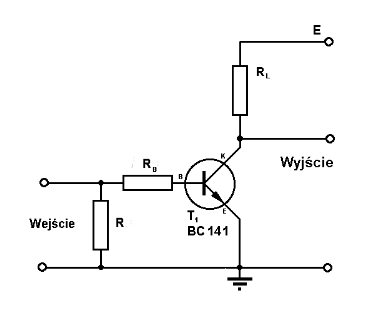
\includegraphics[width = 0.6\textwidth]{obwod1.png}
		\caption{Schematyczny rysunek przedstawiający obwód służący do wykonania pomiarów napięcia w celu zbadania wzmocnienia prądowego \cite{schematy}.}
		\label{obwod1}
	\end{center}
\end{figure}	
Pozwolił on zbadać charakterystykę prądowo napięciową tranzystora. \\
Następnym krokiem doświadczenia było skonstruowanie obwodu przedstawionego na Rys.(\ref{obwod2}).
\begin{figure}[ht!]	
	\begin{center}
		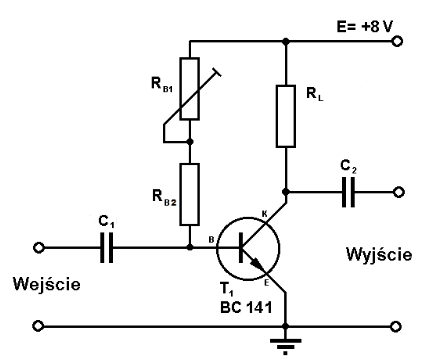
\includegraphics[width = 0.6\textwidth]{obwod2.png}
		\caption{Schematyczny rysunek przedstawiający obwód służący do wykonania pomiarów napięcia w celu zbadania wzmocnienia napięciowego, oraz jego zależności od częstotliwości sygnału wejściowego \cite{schematy}.}
		\label{obwod2}
	\end{center}
\end{figure}	
Przy jego użyciu zmierzono wartości napięcia wejściowego, oraz wyjściowego w tych samych punktach fazy dla częstotliwości sygnału wejściowego $f = 1000 \text{[Hz]}$, a w następnym kroku szczytowe wartości napięć obu sygnałów dla różnych wartości częstotliwości sygnału wejściowego.

\section*{Analiza danych}
\subsection*{Wzmocnienie prądowe}
Pierwszą częścią doświadczenia było sprawdzenie słuszności wzoru (1), czyli wzmocnienia prądowego tranzystora bipolarnego. Posłużył do tego wyżej opisany układ doświadczalny.
\begin{table}[htp!]
\begin{center}
\begin{tabular}{|c|c|c|c|c|}
\hline
 $U_{we}$ [V] & $M_{U_{we}}$ [V] & $E$ [V] & $U_{wy}$ [V] & $M_{U_{wy}}$ \\
\hline
0.5056      & 1                      & 2.52                          & 2.52             & 1                      \\
1.00082     & 1                      & 2.4                           & 2.4              & 1                      \\
2.00249     & 1                      & 2.2                           & 2.44             & 1                      \\
3.001       & 1                      & 2.02                          & 2.4              & 1                      \\
4.0014      & 1                      & 1.84                          & 2.4              & 1                      \\
5.0007      & 1                      & 1.68                          & 2.4              & 1                      \\
6.002       & 1                      & 1.44                          & 2.4              & 1                      \\
7.001       & 1                      & 1.24                          & 2.2              & 1     \\     
\hline  
\end{tabular}
\end{center}
\caption{Wyniki pomiarów części pierwszej doświadczenia.}
\label{czesc1}
\end{table}
Powyższa tabela Tab.(\ref{czesc1}) przedstawia uzyskane wyniki pomiarowe, zatem napięcie $E$, napięcie maksymalne sygnału wejściowego $U_{we}$, podziałka oscyloskopu przy której dokonano pomiaru $M_{U_{we}}$, napięcie maksymalne sygnału wyjściowego $U_{wy}$ wraz podziałka $M_{U_{wy}}$. Na podstawie tych wartości oraz praw Kirkhoffa oraz Ohm'a możemy policzyć $I_B$ oraz $I_C$ według następujących wzorów:
$$ I_C = \frac{U_{we} - \Omega}{R_B}, \qquad I_B = \frac{E-U_{wy}}{R_L}, $$
gdzie $\Omega$ jest napięciem odpowiedzialnym za występowanie progu potencjału wewnątrz tranzystora, a reszta symboli jest zdefiniowana według schematu z Rys.(\ref{obwod1}).
\begin{table}[htp!]
\begin{center}
\begin{tabular}{|c|c|}
\hline
$R$ 						 & 29.938 k$\Omega$ 						\\
$R_L$                     & 234.92 $\Omega$                      \\
$R_B$                     & 329.5 k$\Omega$                       \\
$R_{B2}$                  & 200.192 k$\Omega$                     \\
$R_L$                     & 1553.34 $\Omega$                      \\
$C_1$                     & 48.5 nF                               \\
$C_2$                     & 1.01 $\mu$F        					\\
\hline                   
\end{tabular}
\end{center}
\caption{Zmierzone wartości oporników oraz kondensatorów użytych w doświadczeniu.}
\label{opory}
\end{table}
Zmierzone wartości oporów znajdują się w Tab.(\ref{opory})
Niepewności $\mu_{U_{we}}$ oraz $\mu_{U_{wy}}$ wynikają ze specyfikacji użytego oscyloskopu wynikającej z \cite{niepewnosci} i dane są następującym wzorem:
$$ \mu_{U} = 0.01 \cdot M_U + 0.01 \cdot U + 0.002\text{V}.$$
Do wartości $I_B$ oraz $I_C$ policzonych na podstawie pomiarów z Tab.1 dopasowano przy pomocy języka Python oraz biblioteki SciPy zależność 
$$ I_C = \beta I_B + b, $$
gdzie wyraz $b$ powinien być równy zeru, a reszta zależności wynika ze wzoru (1). Dopasowanie widać na Rys.(\ref{fig_1})
Otrzymano następujące współczynniki:
$$ \beta = 229 \pm 12 \qquad b = 
0.0064 \pm 0.14. $$
Od razu widać, że zero zawiera się w przedziale $[b - \mu_b, b + \mu_b]$, zaś współczynnik $\beta$ według przewidywań teoretycznych powinień być rzędu 100-200. Jest on zatem zbliżony do przewidywań. 
\begin{figure}[ht!]	
	\begin{center}
		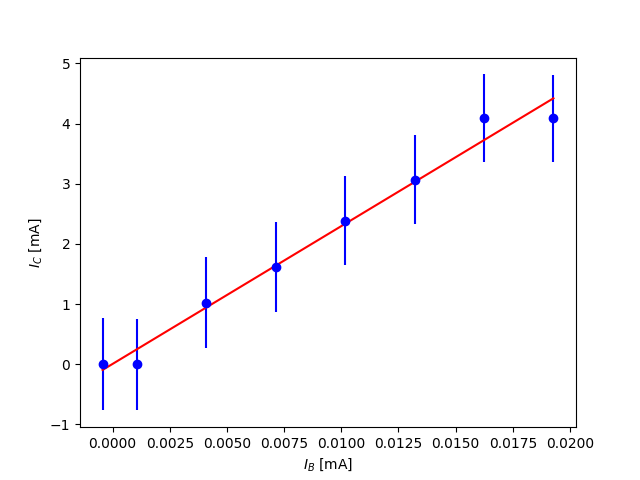
\includegraphics[width = 0.8\textwidth]{Figure_1.png}
		\caption{Obliczone na podstawie pomiarów wartości prądu kolektora $I_C$ oraz bazy $I_B$ wraz z dopasowaniem modelu teoretycznego.}
		\label{fig_1}
	\end{center}
\end{figure}	

\subsection*{Wzmocnienie napięciowe}

\begin{table}[htp!]
\begin{center}
\begin{tabular}{|c|c|c|c|}
\hline
\multicolumn{1}{|l|}{$U_{we}$ {[}V{]}} & \multicolumn{1}{l|}{$\mu_{U_{we}}$ {[}V{]}} & \multicolumn{1}{l|}{$U_{wy}$ {[}V{]}} & \multicolumn{1}{l|}{$\mu_{U_{wy}}$ {[}V{]}} \\ \hline
0.0060                                 & 0.00018                                     & 0.36                                  & 0.011                                       \\
0.01                                   & 0.0003                                      & 0.8                                   & 0.024                                       \\
0.0116                                 & 0.0035                                      & 0.840                                 & 0.025                                       \\
0.0140                                 & 0.00042                                     & 1.04                                  & 0.031                                       \\
0.02                                   & 0.0006                                      & 1.52                                  & 0.046                                       \\
0.0216                                 & 0.00065                                     & 1.64                                  & 0.049                                       \\
0.032                                  & 0.001                                       & 2.48                                  & 0.074                                       \\
0.042                                  & 0.0013                                      & 3.28                                  & 0.1                                         \\
0.054                                  & 0.0016                                      & 4.00                                  & 0.12                                        \\
0.062                                  & 0.0019                                      & 4.8                                   & 0.14                                        \\
0.072                                  & 0.0022                                      & 5.44                                  & 0.16                                        \\
0.082                                  & 0.0025                                      & 6.08                                  & 0.18                                        \\
0.092                                  & 0.0028                                      & 6.64                                  & 0.2                                         \\
0.1                                    & 0.003                                       & 6.69                                  & 0.21                                        \\
0.11                                   & 0.0033                                      & 7.12                                  & 0.21                                        \\
0.118                                  & 0.0035                                      & 7.28                                  & 0.22                                        \\
0.128                                  & 0.0038                                      & 7.440                                 & 0.22                                        \\
0.138                                  & 0.0041                                      & 7.6                                   & 0.23                                        \\
0.146                                  & 0.0044                                      & 7.68                                  & 0.23                                        \\
0.16                                   & 0.0048                                      & 7.8                                   & 0.23                                        \\
0.17                                   & 0.0051                                      & 8.0                                   & 0.24                                        \\
0.18                                   & 0.0054                                      & 8.0                                   & 0.24                                        \\
0.192                                  & 0.0058                                      & 8.0                                   & 0.24                                        \\
0.2                                    & 0.006                                       & 8.0                                   & 0.24        \\
\hline
\end{tabular}
\end{center}
\caption{Wyniki pomiarów drugiej części doświadczenia.}
\label{czesc2}
\end{table}

Na podstawie pomiarów przedstawionych w Tab.(\ref{czesc2}) czyli napięcia maksymalnego sygnału wejściowego $U_{we}$, napięcia maksymalnego sygnału wyjściowego $U_{wy}$ oraz ich niepewności $\mu_{U_{we}}$ i $\mu_{U_{wy}}$ można policzyć współczynnik $k$ ze wzoru (2) dla sygnału wejściowego o częstotliwości $f = 1000 $ [Hz]. Na Rys.(\ref{fig_2}) widać punkty pomiarowe, wraz z niepewnościami, oraz dopasowanie zależności 
$$ U_{wy} = k \cdot U_{we} + b $$ do punktów które układają się w zależność liniową, gdzie tak jak poprzednio, współczynnik $b$ powinien być równy 0. Obliczone (przy użyciu tych samych narzędzi co w punkcie wyżej) parametry wynoszą:
$$ k = 78.9 \pm 1.7 \qquad b = -0.087 \pm 0.023.$$ Do dopasowania wykorzystano $n = 12$ pierwszych punktów pomiarowych. Tym razem zero nie zawiera się w przedziale $[b - \mu_b, b + \mu_b]$, co może wynikać z liniowości tylko fragmentu wykresu oraz trudności w określeniu tego fragmentu. Liczba punktów użytych do dopasowania została wybrana arbitralnie, oceniając zakres liniowości. 
\begin{figure}[ht!]	
	\begin{center}
		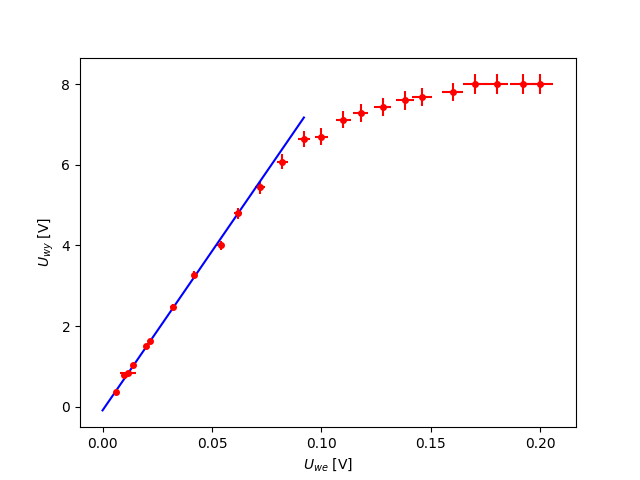
\includegraphics[width = 0.8\textwidth]{Figure_2.png}
		\caption{Pomiary napięcia maksymalnego $U_{we}$ oraz $U_{wy}$ oraz dopasowanie zależności liniowej do pierwszych $n=12$ pomiarów.}
		\label{fig_2}
	\end{center}
\end{figure}	

\subsection*{Zależność wzmocnienia $k(f)$ od częstotliwości}

\begin{table}[htp!]
\begin{center}
\begin{tabular}{|c|c|c|c|c|}
\hline
\multicolumn{1}{|l|}{$f$ {[}Hz{]}} & \multicolumn{1}{l|}{$U_{we}$ {[}V{]}} & \multicolumn{1}{l|}{$\mu_{U_{we}}$ {[}V{]}} & \multicolumn{1}{l|}{$\mu_{U_{wy}}$ {[}V{]}} & \multicolumn{1}{l|}{$\mu_{U_{wy}}$ {[}V{]}} \\ \hline
10                                 & 0.028                                 & 0.00084                                     & 0.12                                        & 0.028                                       \\
25                                 & 0.0264                                & 0.00079                                     & 0.132                                       & 0.026                                       \\
50                                 & 0.0272                                & 0.00082                                     & 0.178                                       & 0.027                                       \\
75                                 & 0.0264                                & 0.00079                                     & 0.244                                       & 0.026                                       \\
100                                & 0.028                                 & 0.00084                                     & 0.32                                        & 0.028                                       \\
200                                & 0.028                                 & 0.00084                                     & 0.6                                         & 0.028                                       \\
500                                & 0.0272                                & 0.00082                                     & 1.22                                        & 0.027                                       \\
750                                & 0.0264                                & 0.00079                                     & 1.7                                         & 0.026                                       \\
1000                               & 0.0272                                & 0.00082                                     & 2.04                                        & 0.027                                       \\
2000                               & 0.0272                                & 0.00082                                     & 2.86                                        & 0.027                                       \\
5000                               & 0.0272                                & 0.00082                                     & 3.36                                        & 0.027                                       \\
7500                               & 0.0272                                & 0.00082                                     & 3.48                                        & 0.027                                       \\
10000                              & 0.0272                                & 0.00082                                     & 3.48                                        & 0.027                                       \\
12000                              & 0.0272                                & 0.00082                                     & 3.48                                        & 0.027                                       \\
15000                              & 0.0272                                & 0.00082                                     & 3.52                                        & 0.027                                       \\
17500                              & 0.0272                                & 0.00082                                     & 3.52                                        & 0.027                                       \\
20000                              & 0.0272                                & 0.00082                                     & 3.48                                        & 0.027                                       \\
50000                              & 0.0272                                & 0.00082                                     & 3.44                                        & 0.027                                       \\
75000                              & 0.0272                                & 0.00082                                     & 3.44                                        & 0.027                                       \\
100000                             & 0.0272                                & 0.00082                                     & 3.44                                        & 0.027                                       \\
250000                             & 0.0272                                & 0.00082                                     & 3.20                                        & 0.027                                       \\
500000                             & 0.0256                                & 0.00077                                     & 2.68                                        & 0.026                                       \\
750000                             & 0.024                                 & 0.00072                                     & 2.16                                        & 0.024                                       \\
1000000                            & 0.0224                                & 0.00067                                     & 1.74                                        & 0.022                                       \\
1100000                            & 0.0224                                & 0.00067                                     & 1.6                                         & 0.022                                       \\
1250000                            & 0.0216                                & 0.00065                                     & 1.44                                        & 0.022                                       \\
1500000                            & 0.0216                                & 0.00065                                     & 1.26                                        & 0.022                  \\
\hline                    
\end{tabular}
\end{center}
\caption{Wyniki pomiarów trzeciej części doświadczenia.}
\label{czesc3}
\end{table}
W tabeli Tab.(\ref{czesc3}) znajdują się wyniki pomiarów trzeciej części doświadczenia. Na ich podstawie, posługując się wzorem (3) można policzyć wzmocnienie dla zadanych częstotliwości. Na Rys.(\ref{fig_3}) przedstawione są wartości wzmocnienia od częstotliwości wraz z niepewnościami. Policzone zostały wykorzystując metodę propagacji małych błędów, która prowadzi do wzoru:
$$ \mu_k = [ (\frac{\mu_{U_{we}}}{U_{wy}})^2 + ( \frac{U_{we}\cdot \mu_{U_{wy}}}{U_{wy}^2} )^2 ]^{\frac{1}{2}}.$$ \\
Na Rys.(\ref{fig_3}) można zauważyć, że dla pewnym częstotliwości współczynnik wzmocnienia jest duży, dla innych marginalny. "Plateau", dla którego współczynnik jest największy nazywamy pasmem przenoszenia. Częstości graniczne dla naszego wzmacniacza zostały ustalone na:
$$ \omega_d = 50 \text{[kHz]}, \qquad \omega_g = 100 \text{[kHz]}, $$
gdzie $\omega_d$ to częstotliwość dolna, zaś $\omega_g$ to częstotliwość górna pasma przenoszenia.

\begin{figure}[ht!]	
	\begin{center}
		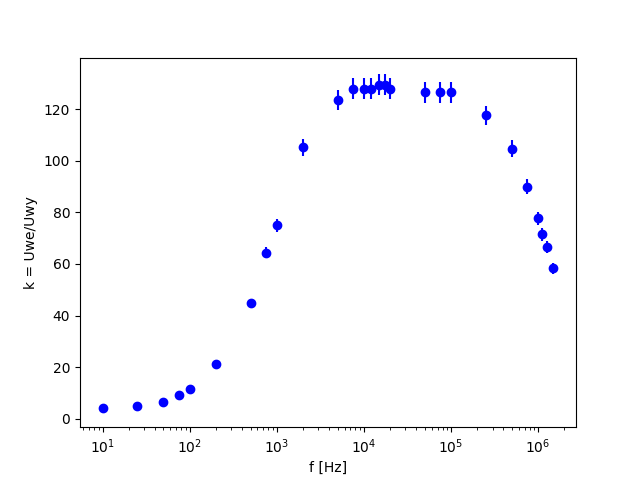
\includegraphics[width = 0.8\textwidth]{Figure_3.png}
		\caption{Wzmocnienie napięciowe dla różnych częstotliwości $f$ sygnału wejściowego, w skali logarytmicznej.}
		\label{fig_3}
	\end{center}
\end{figure}	

\section*{Wnioski}
W ninejszym doświadczeniu udało się zbadać własności tranzystora bipolarnego. Określono, iż natężenie prądu kolektora jest wprost proporcjonalne do natężenia prądu emitera. Dla układu będącego wzmacniaczem tranzystorowym zaś udało się potwierdzić, iż spadek napięcia na kolektorze jest proporcjonalny do napięcia podanego na bazę, aż do punktu krytycznego, przy którym tranzystor się nasyca. Pomyślnie zbadano też charakterystykę częstościową, wyznaczono pasma przenoszenia wzmacniacza. Do wykonania pomiarów użyto oscyloskopu oraz wbudowanej funkcji kursorów, co znacznie zwiększyło dokładność pomiarów. 

\begin{thebibliography}{}
	\bibitem{schematy} Schematy pochodzą z instrukcji do doświadczenia, zostały przerobione w programie graficznym GIMP. http://pracownie1.fuw.edu.pl/pe-A/pliki/Instrukcja%20Tranzystor%202016.pdf
	\bibitem{niepewnosci} Specyfikacja oscyloskopu Rigol DS1000Z-E https://www.batronix.com/files/Rigol/Oszilloskope/DS1000Z-E/DS1000Z-E-Data-sheet.pdf
\end{thebibliography}

\end{document}